\documentclass[12pt]{article}
\usepackage[utf8]{inputenc}

\usepackage[margin=1in]{geometry}

\usepackage{enumerate}
\usepackage{amsmath}
\usepackage{amsfonts}
\usepackage{amssymb}
\usepackage{graphicx}
\usepackage{color}
\usepackage{graphics}
\usepackage{eepic}
\usepackage{nicefrac}
\usepackage{url}
\usepackage{hyperref}
\usepackage{units}
\usepackage{wrapfig}

\usepackage{tikzsymbols}

\usepackage[theoremfont]{newpxtext}
\usepackage[varbb]{newpxmath}

\usepackage[T1]{fontenc}

% useful
\newcommand{\ignore}[1]{}

% complex stuff
\newcommand{\ann}{\operatorname{ann}}
\renewcommand{\Re}{\operatorname{Re}}
\renewcommand{\Im}{\operatorname{Im}}
\newcommand{\Orb}{\operatorname{Orb}}

% reals
\newcommand{\esssup}{\operatorname{ess~sup}}
\newcommand{\essran}{\operatorname{essran}}
\newcommand{\innprod}[2]{\langle #1 | #2 \rangle}
\newcommand{\linnprod}[2]{\langle #1 , #2 \rangle}
\newcommand{\supp}{\operatorname{supp}}
\newcommand{\Nul}{\operatorname{Nul}}
\newcommand{\Ran}{\operatorname{Ran}}
\newcommand{\abs}[1]{\left\lvert {#1} \right\rvert}
\newcommand{\norm}[1]{\left\lVert {#1} \right\rVert}
\newcommand{\sabs}[1]{\lvert {#1} \rvert}
\newcommand{\snorm}[1]{\lVert {#1} \rVert}

% sets (some)
\newcommand{\C}{{\mathbb{C}}}
\newcommand{\R}{{\mathbb{R}}}
\newcommand{\Z}{{\mathbb{Z}}}
\newcommand{\N}{{\mathbb{N}}}
\newcommand{\Q}{{\mathbb{Q}}}
\newcommand{\D}{{\mathbb{D}}}
\newcommand{\F}{{\mathbb{F}}}

% consistent
\newcommand{\bB}{{\mathbb{B}}}
\newcommand{\bC}{{\mathbb{C}}}
\newcommand{\bR}{{\mathbb{R}}}
\newcommand{\bZ}{{\mathbb{Z}}}
\newcommand{\bN}{{\mathbb{N}}}
\newcommand{\bQ}{{\mathbb{Q}}}
\newcommand{\bD}{{\mathbb{D}}}
\newcommand{\bF}{{\mathbb{F}}}
\newcommand{\bH}{{\mathbb{H}}}
\newcommand{\bO}{{\mathbb{O}}}
\newcommand{\bK}{{\mathbb{K}}}
\newcommand{\CP}{{\mathbb{CP}}}
\newcommand{\RP}{{\mathbb{RP}}}
\newcommand{\HP}{{\mathbb{HP}}}
\newcommand{\OP}{{\mathbb{OP}}}
\newcommand{\sA}{{\mathcal{A}}}
\newcommand{\sB}{{\mathcal{B}}}
\newcommand{\sF}{{\mathcal{F}}}
\newcommand{\sG}{{\mathcal{G}}}
\newcommand{\sH}{{\mathcal{H}}}
\newcommand{\sM}{{\mathcal{M}}}
\newcommand{\sO}{{\mathcal{O}}}
\newcommand{\sP}{{\mathcal{P}}}
\newcommand{\sS}{{\mathcal{S}}}
\newcommand{\sI}{{\mathcal{I}}}
\newcommand{\sL}{{\mathcal{L}}}
\newcommand{\sK}{{\mathcal{K}}}
\newcommand{\sU}{{\mathcal{U}}}
\newcommand{\sV}{{\mathcal{V}}}
\newcommand{\sX}{{\mathcal{X}}}
\newcommand{\sY}{{\mathcal{Y}}}
\newcommand{\sZ}{{\mathcal{Z}}}

\newcommand{\interior}{\operatorname{int}}

% Topo stuff
\newcommand{\id}{\textit{id}}
\newcommand{\im}{\operatorname{im}}
\newcommand{\rank}{\operatorname{rank}}
\newcommand{\Tor}{\operatorname{Tor}}
\newcommand{\Torsion}{\operatorname{Torsion}}
\newcommand{\Ext}{\operatorname{Ext}}
\newcommand{\Hom}{\operatorname{Hom}}

%extra thingies
\newcommand{\from}{\ensuremath{\leftarrow}}
\newcommand{\dhat}[1]{\hat{\hat{#1}}}

%\newcommand{\veci}{\hat{\imath}}
%\newcommand{\vecj}{\hat{\jmath}}
%\newcommand{\veck}{\hat{k}}
\newcommand{\veci}{\mathbf{i}}
\newcommand{\vecj}{\mathbf{j}}
\newcommand{\veck}{\mathbf{k}}

% discourage pagebreak at end of display, put before \end{equation}
\newcommand{\avoidbreak}{\postdisplaypenalty=100}

\begin{document}

\title{Calculus III Refresher for Vector Calculus}
\author{Ji\v{r}\'\i{} Lebl}

\maketitle


This class, Vector Calculus, is really the vector calculus that you haven't
really gotten to in Calculus III.
We will be using the book:

\medskip

\noindent
H.\ M.\ Schey,
\emph{Div, Grad, Curl, and All That: An Informal Text on Vector Calculus} (4th Edition)

\medskip

We start with a very quick review of the concepts
from Calculus III that we will
need and that are not covered in Schey---a crash course if you will.
We'll cover nowhere near everything that you may have seen in Calculus III in this quick overview,
just what is needed to read through Schey.
We will also go over a couple of things that you may not have seen
in Calculus III, but that we will need for this class.
You should look back at your Calculus III textbook.  If you no longer have that or need another source, there is a wonderful free textbook:

\medskip

\noindent
Gregory Hartman, \emph{APEX Calculus}, \url{http://www.apexcalculus.com}.  You can download a PDF online, or buy a very cheap printed copy.  Especially Volume 3, that is, chapters 9--14.

%%%%%%%%%%%%%%%%%%%%%%%%%%%%%%%%%%%%%%%%%%%%%%%%%%%%%%%%%%%%%%%%%%%%%%%%%%%%%%%%%%%%%%%%

\section{Points and vectors}

In basic calculus, one deals with $\R$, the real numbers, a one-dimensional space, or the \emph{line}.
In vector calculus, we consider the two-dimensional cartesian space $\R^2$,
the \emph{plane};
three-dimensional space $\R^3$; and in general the $n$-dimensional cartesian space $\R^n$.
A \emph{point} in $\R^2, \R^3$, or $\R^n$ is simply a tuple,
a 3-tuple, or an $n$-tuple (respectively) of real numbers.
For example, the following are points in $\R^2$:
\[
(1,-2), \qquad (0,1), \qquad (-1,10), \qquad \text{etc.}
\]
The following are points in $\R^3$:
\[
(1,-2,3), \qquad (0,0,1), \qquad (-1,-1,10), \qquad \text{etc.}
\]
Of course, $\R^n$ can be $\R^2$ or $\R^3$, and even $\R = \R^1$, as $n$ can always be
1, 2, or 3.
The coordinates used in calculus are often $x$ for $\R$, $(x,y)$ for $\R^2$, and $(x,y,z)$
for $\R^3$.
In $\R^n$, we run out of letters, and so we use something like
subscripts $(x_1,x_2,\ldots,x_n)$.  Letters other than $x$ are also used.
We mostly focus on $\R^3$ (and $\R^2$ to some extent) in this course.

Now that we have points, another object is a \emph{vector}.
A vector is an object that describes a \emph{direction} and a \emph{magnitude} (its size or length).
It is simply an arrow in space that
does not really care where it starts,
it only cares about its direction and its magnitude.

To give vectors names, people often use
$\mathbf{v}$ or $\vec{v}$, although mathematicians often just write $v$ and simply remember
that $v$ is a vector.
On the board, I write $\vec{v}$ although the book uses $\mathbf{v}$
(it is difficult to write bold on the board \Smiley{}).
The book also uses $\hat{\mathbf{v}}$ for unit vectors, that is,
vectors of magnitude one.

\begin{wrapfigure}{r}{0.9in}
\vspace*{-0.1in}
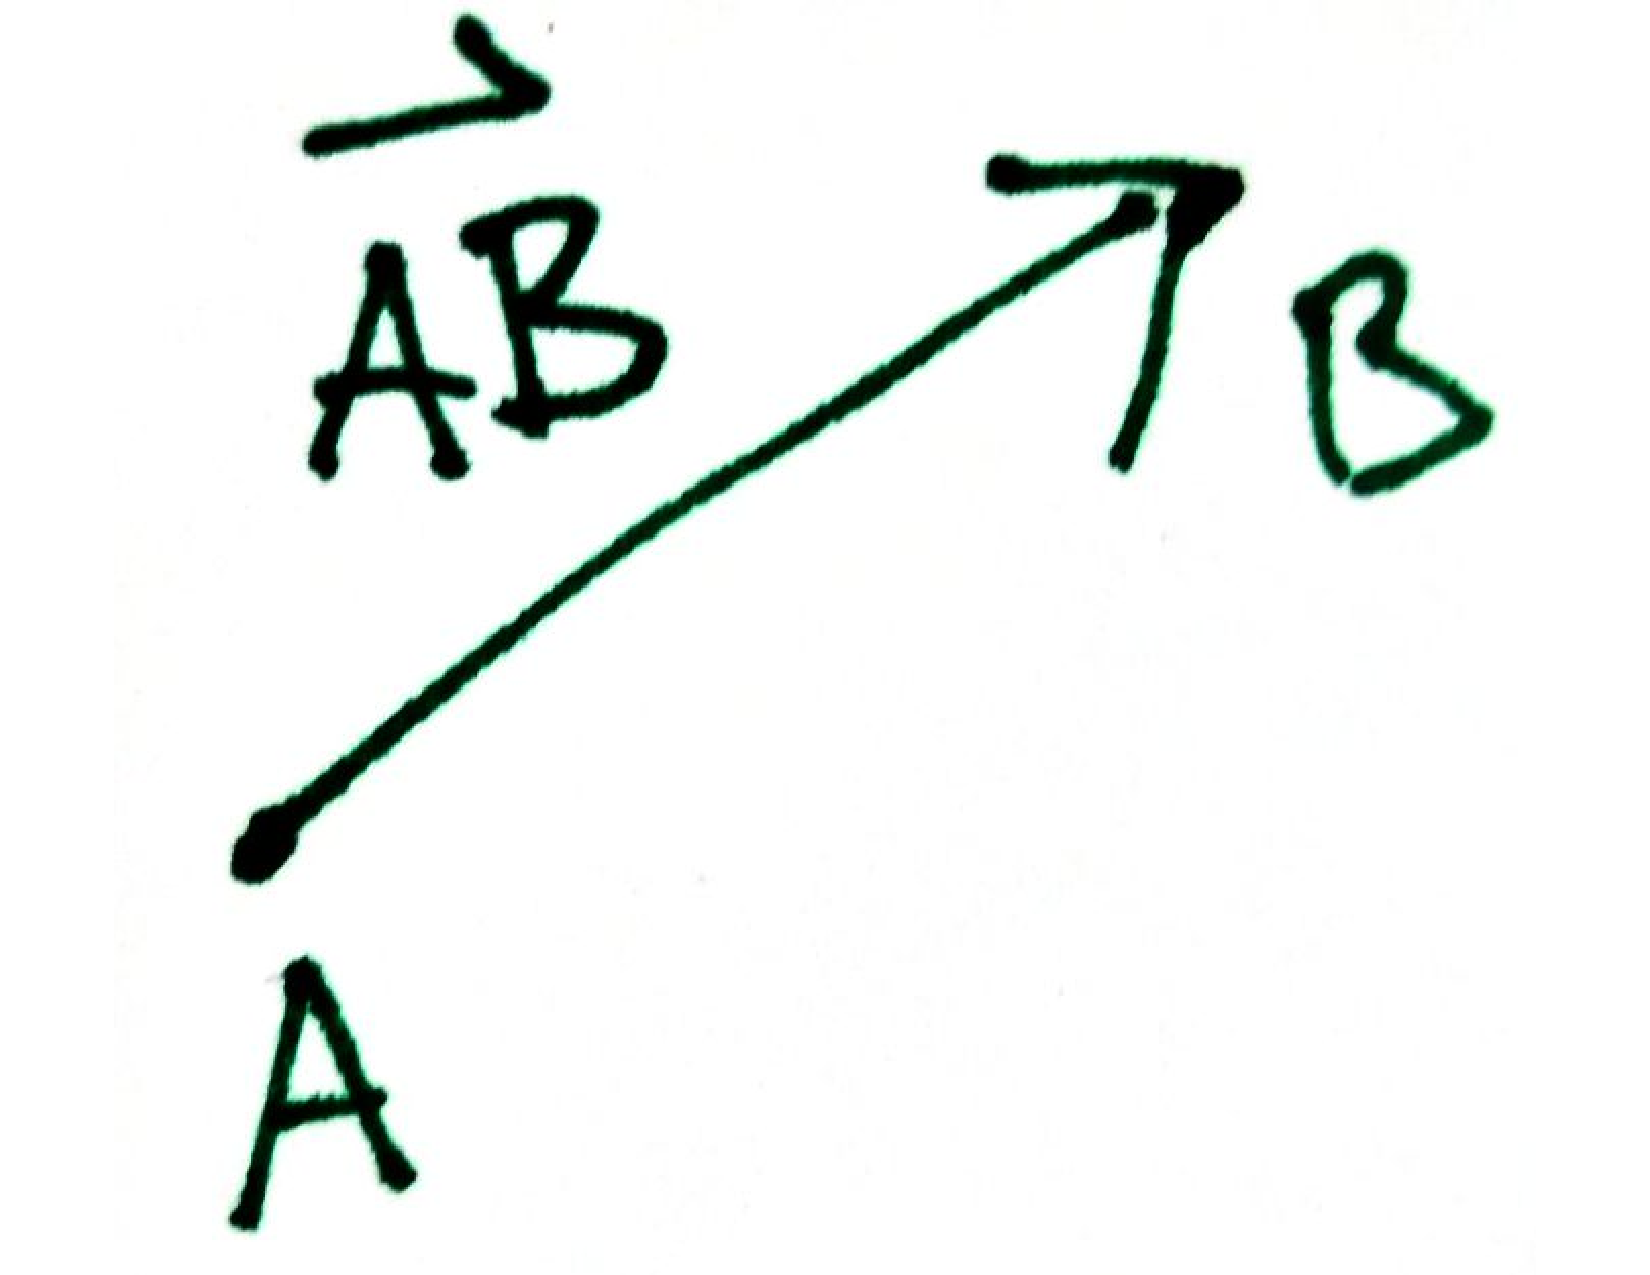
\includegraphics[width=0.9in,page=1]{figures1}
\end{wrapfigure}
The best way to think about it is thinking of a moving particle in space.
A \emph{point} describes the position of a particle,
while a \emph{vector} describes velocity, that is, the direction the object is traveling, and its speed.
Forces and displacements are also described by vectors.
A vector can say how to go from point $A$ to point $B$
(start at $A$ in this direction and go this far to get to $B$).
We write such a vector as $\overrightarrow{AB}$.

The space $\R^n$ has one special point $O = (0,0,\ldots,0)$, the \emph{origin}.
We can describe a vector $\mathbf{v}$ via a point $A$ in space if the vector describes the
displacement from $O$ to $A$, so $\mathbf{v} = \overrightarrow{OA}$.
We say $\mathbf{v}$ is the \emph{position vector} of the point $A$.
This means that a vector can be described by 3 numbers just like a point.
We don't necessarily want to use the same notation as for points.
To distinguish the concepts,
a common notation for vectors is
\[
\langle a,b,c \rangle ,
\]
which is the position vector of the point $(a,b,c)$ in $\R^3$.
Even though both points and vectors are represented by 3 numbers in $\R^3$,
we distinguish them.
As far as computations are concerned,
they are often just 3 numbers, but they are different things.
Just like say temperature, time, or speed are very different
things, they are each described by a single number.  And we don't want to
confuse speed, time, and temperature.

The analogue of the origin is the zero vector $\mathbf{0}$, for example,
\[
\mathbf{0} = \langle 0,0,0 \rangle
\]
in $\R^3$.
It is the single vector that does not have a well-defined direction
and has a zero magnitude.
If you go distance zero, then it doesn't matter in which direction
you travel.

There are certain special vectors called the
\emph{standard basis vectors}.
In $\R^2$ and $\R^3$, they have special names.
In $\R^2$,
\[
\veci = \langle 1 , 0 \rangle, \qquad
\vecj = \langle 0 , 1 \rangle.
\]
In $\R^3$,
\[
\veci = \langle 1, 0, 0 \rangle, \qquad
\vecj = \langle 0, 1, 0 \rangle, \qquad
\veck = \langle 0, 0, 1 \rangle.
\]
Sometimes, people write hats above the ijk,
because these vectors are
unit vectors, but the book doesn't do that, so we will also not do it
here (although I may do so on the board).

A convenient way to write vectors is using the standard basis.
That is, in $\R^2$, write
\[
\langle a,b \rangle = a \veci + b \vecj,
\qquad \text{e.g.,} \quad
\langle 3,4 \rangle = 3 \veci + 4 \vecj.
\]
In $\R^3$, write
\[
\langle a,b,c \rangle = a \veci + b \vecj + c \veck,
\qquad \text{e.g.,} \quad
\langle 3,4,-2 \rangle = 3 \veci + 4 \vecj - 2 \veck.
\]

We also allow arithmetic with vectors.
First, scalar multiplication.
Real numbers are called \emph{scalars} when vectors are around,
because they are used to ``scale'' the vectors.
If $\alpha$ is a scalar and $\mathbf{v}$
is a vector, then the product $\alpha\mathbf{v}$ is the vector with the same direction as
$\mathbf{v}$ (as long as $\alpha \geq 0$) and magnitude multiplied by $\alpha$.
If $\alpha < 0$, then the direction is reversed and the magnitude is multiplied by
$\sabs{\alpha}$.
It turns out that
\[
\alpha ( a \veci + b \vecj + c \veck ) =
\alpha a \veci + \alpha b \vecj + \alpha c \veck,
\qquad \text{e.g.,} \quad
2 ( 3 \veci + 4 \vecj - 2 \veck ) =
6 \veci + 8 \vecj - 4 \veck
.
\]
We can also add vectors.
Vector addition is defined by using the displacement interpretation of vectors.
If $\mathbf{v}$ and $\mathbf{w}$ are vectors,
then $\mathbf{v}+\mathbf{w}$ is the vector where we travel along $\mathbf{v}$ first
and then along $\mathbf{w}$.
It turns out that
\[
( a \veci + b \vecj + c \veck ) +
( d \veci + e \vecj + f \veck ) =
(a+d) \veci + (b+e) \vecj + (c+f) \veck .
\]
E.g.,
\[
( \veci + 2 \vecj + 3 \veck ) +
( 5 \veci + \vecj - 3 \veck ) =
6 \veci + 2 \vecj + 0 \veck = 6 \veci + 2 \vecj
.
\]

We write the magnitude of $\mathbf{v}$ as
$\sabs{\mathbf{v}}$.
The following formulas compute the magnitude of a vector.
In $\R^2$,
\[
\sabs{a \veci + b \vecj}
=
\sqrt{a^2+b^2} ,
\]
and in $\R^3$,
\[
\sabs{a \veci + b \vecj + c \veck}
=
\sqrt{a^2+b^2+c^2} .
\]
Sometimes when given a vector $\mathbf{r}$, its magnitude is written simply as
$r$, rather than $\sabs{\mathbf{r}}$.
You may have seen $\snorm{\mathbf{v}}$ for magnitude. 
It is the same thing.
We will use single bars in this course to
match the book.

The direction of $\mathbf{v}$ written $\hat{\mathbf{v}}$ is then
the vector
\[
\hat{\mathbf{v}} = \frac{1}{\sabs{\mathbf{v}}} \mathbf{v} = \frac{\mathbf{v}}{\sabs{\mathbf{v}}} .
\]
Although we'll try to state explicitly that $\hat{\mathbf{v}}$  is the direction of $\mathbf{v}$.
Notice again that we put a hat on unit vectors, in this case we put a hat
on $\mathbf{v}$ to \emph{make} it into a unit vector.
We often use $\hat{\mathbf{v}}$ for a unit vector even if there was no
$\mathbf{v}$ to begin with.

These notions are generalized to $\R^n$ in the obvious manner.
Higher dimensions do occur naturally.
For example, if $t$ is time, then time-space can have the coordinates $(x,y,z,t)$,
that is $\R^4$.  The space of all configurations of two particles in 3-space
is really $\R^6$, that is $(x_1,y_1,z_1,x_2,y_2,z_2)$, where
$(x_1,y_1,z_1)$ is the position of the first particle and $(x_2,y_2,z_2)$ is
the position of the second.
Similarly, the space of possible
position-velocity configurations (phase space)
of a single particle has 6 dimensions
(3 dimensions for position and 3 for velocity).
And if we are modeling liquid by pretending it
is a thousand particles (liquid, after all,
is a whole bunch of particles),
then the phase space has dimension 6000.

%%%%%%%%%%%%%%%%%%%%%%%%%%%%%%%%%%%%%%%%%%%%%%%%%%%%%%%%%%%%%%%%%%%%%%%%%%%%%%%%%%%%%%%%

\section{Products of vectors}

We saw one product, that is, the product of a scalar and a vector,
$\alpha \mathbf{v}$.
Another type of product is the so-called \emph{dot product}
\[
( a \veci + b \vecj + c \veck ) \cdot
( d \veci + e \vecj + f \veck ) =
ad + be + cf .
\]
E.g.,
\[
( 3 \veci + \vecj -2 \veck ) \cdot
( - 2\veci + 5 \vecj + \veck ) =
-6 + 5 -2 = -3 .
\]
This product is easy to generalize to any number of dimensions in the obvious way.
Notice that the result of this product is a scalar and not a vector.
For this reason, it is sometimes called the scalar product.
The dot product can compute the magnitude of a vector:
\[
\sabs{\mathbf{v}}^2 = \mathbf{v} \cdot \mathbf{v} .
\]
\begin{wrapfigure}[4]{r}{1.0in}
\vspace*{-0.35in}
\includegraphics[width=1.0in,page=2]{figures1}
\end{wrapfigure}
Geometrically in $\R^2$ or $\R^3$, this product is
\[
\mathbf{v} \cdot \mathbf{w} = \sabs{\mathbf{v}} \sabs{\mathbf{w}} \cos \theta ,
\]
where $\theta$ is the angle between $\mathbf{v}$ and $\mathbf{w}$.
So the dot product can be used to compute the angle.
It doesn't matter if you think of the angle
between $\mathbf{v}$ and $\mathbf{w}$ or vice-versa, as we are taking the cosine here:
There are two ways you could define the angle depending on which direction you start in,
but because of the cosine you get the same dot product.
Two vectors are \emph{orthogonal}
(at right angle, perpendicular) if their dot product is zero.

The dot product is bilinear (if something is called a product, usually people want it to be bilinear):
\[
( \alpha \mathbf{v} + \beta \mathbf{w} ) \cdot \mathbf{u}
=
\alpha (\mathbf{v} \cdot \mathbf{u}) + \beta (\mathbf{w} \cdot \mathbf{u})
\]
and
\[
\mathbf{u} \cdot
( \alpha \mathbf{v} + \beta \mathbf{w} )
=
\alpha (\mathbf{u} \cdot \mathbf{v}) + \beta (\mathbf{u} \cdot \mathbf{w}) .
\]
It is also commutative (not all products are commutative):
\[
\mathbf{v} \cdot \mathbf{w} = \mathbf{w} \cdot \mathbf{v} .
\]

\begin{wrapfigure}{r}{1.2in}
\vspace*{-0.2in}
\includegraphics[width=1.2in,page=3]{figures1}
\end{wrapfigure}
Another type of product, which really only exists in $\R^3$, is the
\emph{cross product},
sometimes called the \emph{vector product}.
This product results in a vector.
Geometrically
\[
\mathbf{v} \times \mathbf{w} = \sabs{\mathbf{v}} \sabs{\mathbf{w}} (\sin \theta) \hat{\mathbf{n}} ,
\]
where $\theta$ is the angle going from $\mathbf{v}$ to $\mathbf{w}$ in the plane spanned by them
(now the order matters),
and $\hat{\mathbf{n}}$ is the normal vector to that plane oriented according to the right-hand rule.
The orientation can be figured out from the formula
\[
\veci \times \vecj = \veck .
\avoidbreak
\]
That is, $\veck$ is the normal vector to the $xy$-plane using the right-hand rule.

There are a bunch of ways to compute the cross product, though perhaps the easiest to remember
is using algebra.
First, the cross product is bilinear:
\[
( \alpha \mathbf{v} + \beta \mathbf{w} ) \times \mathbf{u}
=
\alpha (\mathbf{v} \times \mathbf{u}) + \beta (\mathbf{w} \times \mathbf{u})
\]
and
\[
\mathbf{u} \times
( \alpha \mathbf{v} + \beta \mathbf{w} )
=
\alpha (\mathbf{u} \times \mathbf{v}) + \beta (\mathbf{u} \times \mathbf{w}) .
\]
It is anti-commutative:
\[
\mathbf{v} \times \mathbf{w} = - \mathbf{w} \times \mathbf{v} .
\]
Anticommutativity implies
\[
\mathbf{v} \times \mathbf{v} = \mathbf{0} .
\]
To compute the product, we can use the identities
\[
\veci \times \vecj = \veck , \qquad
\vecj \times \veck = \veci , \qquad
\veck \times \veci = \vecj .
\]
All three identities list $\veci$, $\vecj$, $\veck$ in the same order.
If you go in the opposite order, you get a minus sign:
\[
\vecj \times \veci = -\veck , \qquad
\veck \times \vecj = -\veci , \qquad
\veci \times \veck = -\vecj .
\]

Example:
\[
(3 \veci + \veck) \times (\vecj + 2 \veck)
=
3 \veci \times \vecj + (3 \cdot 2) \veci \times \veck
+
\veck \times \vecj + 2 \veck \times \veck
=
3 \veck + 6 ( - \vecj)
+
(-\veci) + 2 \mathbf{0}
=
-\veci - 6\vecj + 3 \veck .
\]

A very important property of the cross product is that it is orthogonal
to both of the vectors.
In terms of the dot product:
\[
\mathbf{v} \cdot (\mathbf{v} \times \mathbf{w}) = 0 , \qquad
\mathbf{w} \cdot (\mathbf{v} \times \mathbf{w}) = 0 .
\]
It is a useful, easy-to-compute way to find a vector orthogonal to a plane.
For example, as we computed above
$(3 \veci + \veck) \times (\vecj + 2 \veck)
=
-\veci - 6\vecj + 3 \veck$, so
$-\veci - 6\vecj + 3 \veck$ is orthogonal
(at right angle) to 
$3 \veci + \veck$ and also to
$\vecj + 2 \veck$.

A common trick to compute the cross product
is the determinant formula:
\[
(a \veci + b \vecj + c \veck ) \times 
(d \veci + e \vecj + f \veck ) =
\det
\begin{bmatrix}
\veci & \vecj & \veck \\
a & b & c \\
d & e & f
\end{bmatrix}
=
(bf-ce) \veci -
(af-cd) \vecj +
(ae-bd) \veck .
\]
(Do not forget the minus sign on the $\vecj$.)

Perhaps the correct way to define cross product,
and also a way to figure out many of its properties from
the properties of the dot product and
the determinant is the \emph{triple product}.
Let $\mathbf{u} = u_1 \veci + u_2 \vecj + u_3 \veck$,
$\mathbf{v} = v_1 \veci + v_2 \vecj + v_3 \veck$, and
$\mathbf{w} = w_1 \veci + w_2 \vecj + w_3 \veck$.  Then
\[
\mathbf{u} \cdot ( \mathbf{v} \times \mathbf{w} )
=
\det
\begin{bmatrix}
u_1 & u_2 & u_3 \\
v_1 & v_2 & v_3 \\
w_1 & w_2 & w_3
\end{bmatrix} .
\]

%%%%%%%%%%%%%%%%%%%%%%%%%%%%%%%%%%%%%%%%%%%%%%%%%%%%%%%%%%%%%%%%%%%%%%%%%%%%%%%%%%%%%%%%

\section{Functions and partial derivatives}

A function is simply an assignment of inputs to some output.
A real-valued\footnote{By \emph{real} we mean the real numbers,
as opposed to complex numbers, which we will not worry about.}
function of 3 real variables can be written as
\[
w = f(x,y,z) .
\]
That is, given numbers $x$, $y$, and $z$, the function $f$ returns the number $f(x,y,z)$.
For example, if $x$, $y$, $z$ are some coordinates on our classroom,
then the temperature $T(x,y,z)$ at any particular point in the room
is a function.  Sometimes, a scalar-valued function is called a
``scalar function'' or a ``scalar field.''

If we keep $y$ and $z$ fixed, then the assignment that takes $x$ to $f(x,y,z)$ is a
function of one variable.
Its derivative is the so-called \emph{partial derivative} with respect to $x$,
written $\frac{\partial f}{\partial x}$.  That is,
\[
\frac{\partial f}{\partial x}(x,y,z) =
\lim_{h\to 0} \frac{f(x+h,y,z)-f(x,y,z)}{h} .
\]
Similarly, we define
$\frac{\partial f}{\partial y}$,
$\frac{\partial f}{\partial z}$ and so on.  These partial derivatives are again
functions of $\R^3$.
We will not use the notation $f_x$ in this
course for the partial derivative as
it may get confusing;
we reserve the subscript for another concept.

To compute partials, we simply consider all other variables constant.
For example, if $f(x,y,z) = x^2yz + xy + z$, then
\[
\frac{\partial f}{\partial x}(x,y,z) = 2xyz + y,
\qquad
\frac{\partial f}{\partial y}(x,y,z) = x^2z + x,
\qquad \text{and} \qquad
\frac{\partial f}{\partial z}(x,y,z) = x^2y + 1 .
\]
As these are functions, we may take the derivative again.  Let us show a couple of examples,
\[
\frac{\partial^2 f}{\partial x \partial y}(x,y,z) = 2xz + 1,
\qquad \text{and} \qquad
\frac{\partial^2 f}{\partial x^2}(x,y,z) = 2yz .
\]

The generalization to $n$ variables is similar.  E.g.,
if $f(x_1,x_2,x_3,x_4) = x_1^2x_2x_3 + x_2 x_4$, then
\[
\frac{\partial f}{\partial x_1}(x_1,x_2,x_3,x_4) = 2x_1 x_2 x_3,
\qquad \text{or} \qquad
\frac{\partial f}{\partial x_2}(x_1,x_2,x_3,x_4) = x_1^2 x_3 + x_4 .
\]

\section{Multidimensional integrals}

\begin{wrapfigure}[6]{r}{1.2in}
\vspace*{-0.4in}
\includegraphics[width=1.2in,page=4]{figures1}
\end{wrapfigure}
In the plane, the area of a small rectangle with sides $\Delta x$ and $\Delta y$
is $\Delta A = \Delta x \Delta y$.
If we build a box of height $c$ above
this small rectangle, the volume of the box is $c \Delta x \Delta y = c \Delta A$.

Let $R = [a,b] \times [c,d]$ be a rectangle in $\R^2$, and suppose
$f$ is a function of two variables defined for values in $R$.
That is, $R$ is all the points
$(x,y)$ such that $a \leq x \leq b$ and $c \leq y \leq d$,
and for every $(x,y)$ in $R$ we have a value $f(x,y)$.
We divide $R$ into a bunch of rectangles of area $\Delta A = \Delta x \Delta y$.
In each of these rectangles, we pick a point $(x_j,y_j)$.  Then
\[
f(x_j,y_j) \Delta A
\]
is a reasonable approximation for the volume under the graph of $f$ above the little
rectangle.
We sum all these approximations
\[
\sum_j 
f(x_j,y_j) \Delta A .
\]
This sum is
a reasonable approximation for the volume under the graph of $f$ above the rectangle
$R$.
The double integral of $f$ over $R$ is the limit of
this expression
as $\Delta x$ and $\Delta y$ go to zero,
and therefore as $\Delta A$ goes to zero:
\[
\iint_R f(x,y) \, dA =
\lim_{\substack{\Delta x \to 0 \\ \Delta y \to 0}}
\sum_j 
f(x_j,y_j) \Delta A ,
\]
For a reasonable function (e.g.,\ continuous), this limit exists.
The sum can be done column-wise or row-wise, resulting in a
double sum (first over rows and then over columns or vice-versa).
Taking the limits, we find that
\[
\iint_R f(x,y) \, dA
=
\int_c^d \int_a^b f(x,y) \, dx \, dy
=
\int_a^b \int_c^d f(x,y) \, dy \, dx .
\]
Notice the units of this quantity.  It is the units of $f$ times the units of $x$ times
the units of $y$.  So for example, if all three are meters, $\unit{m}$,
then the unit of $dA$ is $\unit{m^2}$ and
the unit of
$f(x,y) \, dA$
and therefore of
$\iint_R f(x,y) \, dA$
is $\unit{m^3}$ or volume.

Let's compute a couple of examples.
First,
\[
\iint_R dA = A(R) = (b-a)(d-c) .
\]
Here $A(R)$ is the area of $R$.
(Note that the units work out as the 
the quantity under the integral, $dA$, has units of area.)
Another example:  Let $R = [0,1] \times [0,1]$
\[
\iint_R xy\, dA =
\int_0^1 \int_0^1 xy \, dx \, dy
=
\int_0^1 \frac{1}{2} y \, dy
= \frac{1}{4}.
\]

Similarly in $\R^3$, a little box of sides $\Delta x$, $\Delta y$, and $\Delta z$
is of volume $\Delta V = \Delta x \Delta y \Delta z$.  
Let $B = [a,b] \times [c,d] \times [e,f]$ be a box.
Given a function $f(x,y,z)$
defined on the box $B$, we follow
the same procedure as above to find the integral
\[
\iiint_B f(x,y,z) \, dV
=
\int_e^f \int_c^d \int_a^b f(x,y,z) \, dx \, dy \, dz .
\]
All the other orderings of $dx$, $dy$, and $dz$ also work.
Notice the units.  If all dimensions, including that of $f$, are in meters, then
the unit of
$\iiint_B f(x,y,z) \, dV$ is $\unit{m^4}$, or 4-dimensional volume,
as the unit of $f$ is $\unit{m}$ and the unit of $dV$ is $\unit{m^3}$.
If on the other hand the units of $f$ are say density $\unitfrac{kg}{m^3}$,
and the units of $x,y,z$ are all meters,
then the unit of
$\iiint_B f(x,y,z) \, dV$ is $\unit{kg}$ as the meters cubed cancel out.

Sometimes, for simplicity, we might just write
\[
\iint_R f \, dA
\quad \text{or} \quad
\iiint_B f \, dV
\avoidbreak
\]
for double or triple integrals.

We could generalize all this further. Given $f(x_1,\ldots,x_n)$ on $\R^n$, we start with
the $n$-dimensional volume element $dV_n$ or just $dV$.
We integrate $f$ and obtain
$(n+1)$-dimensional volume ``under the graph.''
Mathematicians sometimes do not make a distinction for $n=1$ and $n=2$ and simply call
everything ``volume.''
So 1-dimensional volume is length, 2-dimensional volume is
area, etc.
Mathematicians also often do not use $\iint$ and $\iiint$,
and so on, and simply use $\int$,
as we all know the dimension based on the nature of
the element $dV$ or $dA$ or the dimension of the
set, $R$ or $B$, we are integrating over.

An integral over a region that is not a rectangle
is achieved by setting the function to zero
outside this region and then integrating over
a large rectangle.  It can also be achieved by
using iterated integrals and
changing the limits as appropriate.  For example,
given a triangle $T$ with vertices at $(0,0)$, $(2,0)$,
and $(2,1)$, let's compute the integral of $x^2y$
over $T$.  Describe $T$ as either
$0 \leq x \leq 2$, $0 \leq y \leq \frac{x}{2}$, or as
$0 \leq y \leq 1$, $2y \leq x \leq 2$.  Compute
\[
\iint_T x^2 y \, dA
=
\int_0^2 \int_0^{x/2} x^2y \, dy \, dx
=
\int_0^2 x^2\frac{(x/2)^2}{2}  \, dx
=
\int_0^2 \frac{x^4}{8}  \, dx
=
 \frac{2^5}{8 \cdot 5} = \frac{4}{5} ,
\]
or
\[
\iint_T x^2 y \, dA
=
\int_0^1 \int_{2y}^{2} x^2y \, dx \, dy
=
\int_0^1 \left(\frac{2^3 y}{3} - \frac{(2y)^3y}{3} \right) \, dy
=
\int_0^1 \frac{8y-8y^4}{3} \, dy
=
\frac{4}{5} .
\avoidbreak
\]
Not surprisingly, we got the same answer, of course, since it is the same region.

The integral is \emph{additive}, that is, if $R$ is the disjoint union of $R_1$ and $R_2$,
then
\[
\iint_R f \, dA = 
\iint_{R_1} f \, dA +
\iint_{R_2} f \, dA .
\]
The integral is also \emph{linear}, that is, if $\alpha, \beta$ are real numbers and
$f$ and $g$ are functions, then
\[
\iint_R (\alpha f + \beta g) \, dA = 
\alpha \iint_R f \, dA +
\beta \iint_R g \, dA .
\]

Understanding the development of the integral as a sum is important
in applications for recognizing quantities computed by integration.
Only after we recognize that something is an integral can we write the integral as an iterated
one and compute it with the techniques of calculus.
In fact, because calculus is
so powerful, sometimes the approximation goes the other way.
Instead of the sum being an approximation for the integral, the integral can be
computed to approximate a sum.
In some sense, this is always the case, as our world is
really composed of tiny bits rather than continuous unbroken things.
Curiously, adding up a finite but large number of bits tends to be far harder to do than
``adding up infinitely many,'' that is, integrating.
A recurring theme in mathematics is that by making a problem more complicated
(in just the right way), we turn an impossible-to-solve problem
into a tractable, solvable problem.

\end{document}
